\documentclass[fleqn,portrait,final,a0paper]{baposter}
%\documentclass[a4shrink,portrait,final]{baposter}
% Usa a4shrink for an a4 sized paper.

\tracingstats=2

% special 
\usepackage{ifthen}
\usepackage{ifpdf}
\usepackage{float}
\usepackage{color}

% fonts
\usepackage{latexsym}
\usepackage{amsmath} 
\usepackage{amssymb} 
\usepackage{bm}
\usepackage{wasysym}


\ifpdf
\usepackage{graphicx}
\usepackage{epstopdf}
\else
\usepackage{graphicx}
\usepackage{epsfig}
\fi


\graphicspath{{figures/},{PROG/figures/}}


%%%%%%%%%%%%%%%%%%%%%%%%%%%%%%%%%%%%%%%%%%%%%%%%%%%%%%%%%%%%%%%%


% NEW 
\newcommand{\abs}[1]{\left|#1\right|}
\newcommand{\Prob}{\mbox{Prob}\,}
\newcommand{\erf}{\mbox{erf}\,}
\newcommand{\barline}[1]{#1}

% math symbols I
\newcommand{\sinc}{\mbox{sinc}}
\newcommand{\const}{\mbox{const}}
\newcommand{\trc}{\mbox{trace}}
\newcommand{\intt}{\int\!\!\!\!\int }
\newcommand{\ointt}{\int\!\!\!\!\int\!\!\!\!\!\circ\ }
\newcommand{\ar}{\mathsf r}
\newcommand{\im}{\mbox{Im}}
\newcommand{\re}{\mbox{Re}}

% math symbols II
\newcommand{\eexp}{\mbox{e}^}
\newcommand{\bra}{\left\langle}
\newcommand{\ket}{\right\rangle}

% Mass symbol
\newcommand{\mass}{\mathsf{m}} 
\newcommand{\Mass}{\mathsf{M}} 

% more math commands
\newcommand{\tbox}[1]{\mbox{\tiny #1}}
\newcommand{\bmsf}[1]{\bm{\mathsf{#1}}} 
%\newcommand{\amatrix}[1]{\matrix{#1}} 
\newcommand{\amatrix}[1]{\begin{matrix} #1 \end{matrix}} 
\newcommand{\pd}[2]{\frac{\partial #1}{\partial #2}}

% equations
\newcommand{\mylabel}[1]{\label{#1}} 
%\newcommand{\mylabel}[1]{\textcolor{blue}{[#1]}\label{#1}} 
\newcommand{\beq}{\begin{eqnarray}}
\newcommand{\eeq}{\end{eqnarray}} 
\newcommand{\be}[1]{\begin{eqnarray}\ifthenelse{#1=-1}{\nonumber}{\ifthenelse{#1=0}{}{\mylabel{e#1}}}}
\newcommand{\ee}{\end{eqnarray}} 

% arrangement
\newcommand{\drawline}{\begin{picture}(500,1)\line(1,0){500}\end{picture}}
\newcommand{\bitem}{$\bullet$ \ \ \ }
\newcommand{\Cn}[1]{\begin{center} #1 \end{center}}
\newcommand{\mpg}[2][1.0\hsize]{\begin{minipage}[b]{#1}{#2}\end{minipage}}
\newcommand{\mpgt}[2][1.0\hsize]{\begin{minipage}[t]{#1}{#2}\end{minipage}}
\newcommand{\putgraph}[2][width=0.30\hsize]{\includegraphics[#1]{#2}}

% more
%\newcommand{\Eq}[1]{Eq.\!\!~(\ref{#1})}
%\newcommand{\Fig}[1]{Fig.\!\!~\ref{#1}}  
\newcommand{\Eq}[1]{\textcolor{blue}{Eq.\!\!~(\ref{#1})}} 
\newcommand{\Fig}[1]{\textcolor{blue}{Fig.}\!\!~\ref{#1}} 
\newcommand{\hide}[1]{} %{\textcolor{red}{[hidden text]}} %{}
\newcommand{\rmrk}[1]{\textcolor{red}{#1}}


%%%%%%%%%%%%%%%%%%%%%%%%%%%%%%%%%%%%%%%%%%%%%%%%%%%%%%%%%%%%%%%%%%%%%%%%%%%

% extra math commands by jarondl
\newcommand{\inner}[2]{\left \langle #1 \middle| #2\right\rangle} % Inner product
\newcommand{\avgangle}[1]{\left\langle #1 \right\rangle} % Average <x>

%fminipage using fancybox package
\newenvironment{fminipage}%
  {\begin{Sbox}\begin{minipage}}%
  {\end{minipage}\end{Sbox}\fbox{\TheSbox}}

%%%%% REMOVING the bibliography title
\renewcommand{\refname}{}


\mathindent=0.0pt

%%%%%%%%%%%%%%%%%%%%%%%%%%%%%%%%%%%%%%%%%%%%%%%%%%%%%%%%%%%%%%%%%%%%%%%%%%%%%%
%%% Begin of Document
%%%%%%%%%%%%%%%%%%%%%%%%%%%%%%%%%%%%%%%%%%%%%%%%%%%%%%%%%%%%%%%%%%%%%%%%%%%%%%

\begin{document}

%%%%%%%%%%%%%%%%%%%%%%%%%%%%%%%%%%%%%%%%%%%%%%%%%%%%%%%%%%%%%%%%%%%%%%%%%%%%%%
%%% Here starts the poster
%%%---------------------------------------------------------------------------
%%% Format it to your taste with the options
%%%%%%%%%%%%%%%%%%%%%%%%%%%%%%%%%%%%%%%%%%%%%%%%%%%%%%%%%%%%%%%%%%%%%%%%%%%%%%
% Define some colors
\definecolor{silver}{cmyk}{0,0,0,0.3}
\definecolor{yellow}{cmyk}{0,0,0.9,0.0}
\definecolor{reddishyellow}{cmyk}{0,0.22,1.0,0.0}
\definecolor{black}{cmyk}{0,0,0.0,1.0}
\definecolor{darkYellow}{cmyk}{0,0,1.0,0.5}
\definecolor{darkSilver}{cmyk}{0,0,0,0.1}

\definecolor{lightyellow}{cmyk}{0,0,0.3,0.0}
\definecolor{lighteryellow}{cmyk}{0,0,0.1,0.0}
\definecolor{lighteryellow}{cmyk}{0,0,0.1,0.0}
\definecolor{lightestyellow}{cmyk}{0,0,0.05,0.0}

%%
%\background{
%  \begin{tikzpicture}[remember picture,overlay]%
%    \draw (current page.north west)+(-2em,2em) node[anchor=north west] {\includegraphics[height=1.1\textheight]{silhouettes_background}};
%  \end{tikzpicture}%
%}
\typeout{Poster Starts}



\begin{poster}%
  % Poster Options
  {
  bgColorOne=lightgray!30,
  %bgColorTwo=yellow,
  headerheight=0.1\textheight,
  columns=3,
  headershade=plain,
  headerColorOne=green!40,
  boxColorOne=lightgray!75,
  headershape=smallrounded,
  textborder=roundedsmall,
  linewidth=0.5pt,
  borderColor=green,
  headerborder=open,
  eyecatcher=false,
  background=plain
}
  % Eye Catcher
  {\includegraphics[width=10em]{D1077}} % No eye catcher for this poster. (eyecatcher=no above). If an eye catcher is present, the title is centered between eye-catcher and logo.
  % Title
  {\bf \vspace{1em}\center{
Transport in "sparse" networks:\\ 
\hspace{1em}From linear response to effective range hopping.}}
  % Authors
  {\sf
  \vspace{-1.2em}  {\center{Yaron de Leeuw, Doron Cohen\\
Ben-Gurion University of the Negev\\}}
%                Physics Department \\
%                 Ben-Gurion University of the Negev, \\
%                Beer-Sheva, Israel\\
%                \texttt{jarondl@bgu.ac.il}}
  }
  % University logo
  {\hspace{1em}
\includegraphics[height=10em]{BGU}\
  }

  \tikzstyle{light shaded}=[top color=baposterBGtwo!30!white,bottom color=baposterBGone!30!white,shading=axis,shading angle=30]


%%%%%%%%%%%%%%%%%%%%%%%%%%%%%%%%%%%%%%%%%%%%%%%%%%%%%%%%%%%%%%%%%%%%%%%%%%%%%%
%%% Now define the boxes that make up the poster
%%%---------------------------------------------------------------------------
%%% Each box has a name and can be placed absolutely or relatively.
%%% The only inconvenience is that you can only specify a relative position 
%%% towards an already declared box. So if you have a box attached to the 
%%% bottom, one to the top and a third one which should be in between, you 
%%% have to specify the top and bottom boxes before you specify the middle 
%%% box.
%%%%%%%%%%%%%%%%%%%%%%%%%%%%%%%%%%%%%%%%%%%%%%%%%%%%%%%%%%%%%%%%%%%%%%%%%%%%%%
%%%%%%%%%%%%%%%%%%%%%%%%%%%%%%%%%%%%%%%%%%%%%%%%%%%%%%%%%%%%%%%%%%%%%%%%%%%%%%
  \headerbox{References}{name=refs,column=1,span=2,above=bottom}{
%%%%%%%%%%%%%%%%%%%%%%%%%%%%%%%%%%%%%%%%%%%%%%%%%%%%%%%%%%%%%%%%%%%%%%%%%%%%%%
\vspace{-1em}
{\small
\begin{thebibliography}{99}
\bibitem{alexander}
S. Alexander, J. Bernasconi, W.R. Schneider, R. Orbach, 
Rev. Mod. Phys. 53, 175 (1981).

\bibitem{amir} 
A. Amir, Y. Oreg, Y. Imry,
Phys. Rev. Lett. 105, 070601 (2010); 
%
Phys. Rev. B 77, 165207 (2008).

\bibitem{kbd} 
A. Stotland, T. Kottos, D. Cohen, 
Phys. Rev. B  81, 115464 (2010).

%\bibitem{miller}
%A. Miller and E. Abrahams, Phys. Rev. {\bf 120}, 745 (1960).

\end{thebibliography}

}
}
%%%%%%%%%%%%%%%%%%%%%%%%%%%%%%%%%%%%%%%%%%%%%%%%%%%%%%%%%%%%%%%%%%%%%%%%%%%%%%


%%%%%%%%%%%%%%%%%%%%%%%%%%%%%%%%%%%%%%%%%%%%%%%%%%%%%%%%%%%%%%%%%%%%%%%%%%%%%%
  \headerbox{The model}{name=model,column=0,row=0}{
%%%%%%%%%%%%%%%%%%%%%%%%%%%%%%%%%%%%%%%%%%%%%%%%%%%%%%%%%%%%%%%%%%%%%%%%%%%%%%
{}

Motivated by \cite{alexander,amir,kbd}, we consider 1D, quasi-1D and 2D networks with:
\begin{align*}
\frac{dp_n}{dt} \quad=\quad \sum_m w_{nm} p_m
\end{align*}
The random site model ($1D$ / $2D$ ) : %\cite{amir}:
\begin{align*}
w_{nm} \quad&=\quad  w_0\eexp{-\epsilon_{nm}}\eexp{-|x_n-x_m|/\xi}  \\
x_n \quad&=\quad \mbox{random with avg. distance $r_0$}\\
s \quad&\equiv\quad \xi/r_0\\
\epsilon_{nm} \quad&=\quad \mbox{random activation potential} \in [0,\sigma] 
\end{align*}
%
The banded lattice model (quasi-$1D$ ) : %\cite{kbd}:
%
\begin{align*}
w_{nm}  \quad&=\quad   w_0  \eexp{-\epsilon_{nm}}  B(n-m) \\
b \quad&=\quad \mbox{"bandwidth"}\quad = \quad\mbox{width of }\  B(r)
\end{align*}


}
%%%%%%%%%%%%%%%%%%%%%%%%%%%%%%%%%%%%%%%%%%%%%%%%%%%%%%%%%%%%%%%%%%%%%%%%%%%%%%
  \headerbox{Diffusion}{name=diffusion,column=0, below=model}{
%%%%%%%%%%%%%%%%%%%%%%%%%%%%%%%%%%%%%%%%%%%%%%%%%%%%%%%%%%%%%%%%%%%%%%%%%%%%%%
{}

The long time dynamics are characterized by the spreading $S(t)$, the survival probability $\mathcal{P}(t)$ and the spectral counting function $\mathcal{N}(\lambda)$. In the case of diffusion these are:
\begin{align*}
S(t) \quad&=\quad \left\langle r^2(t)\right\rangle \quad\sim\quad  (2d)Dt\ \\
\mathcal{P}(t) \quad &\sim \quad  \frac{1}{\left({D t}\right)^{d/2}} \\
\mathcal{N}(\lambda)  \quad&\sim\quad \left[\frac{\lambda}{D}\right]^{d/2} 
\end{align*}

 }

%%%%%%%%%%%%%%%%%%%%%%%%%%%%%%%%%%%%%%%%%%%%%%%%%%%%%%%%%%%%%%%%%%%%%%%%%%%%%%
  \headerbox{The $1D$ chain model}{name=chain,column=0,below=diffusion}{
%%%%%%%%%%%%%%%%%%%%%%%%%%%%%%%%%%%%%%%%%%%%%%%%%%%%%%%%%%%%%%%%%%%%%%%%%%%%%%
For $s>1$ we get:
\begin{align*}
D \quad = \quad \left( \frac{1}{N} \sum_n \frac{1}{w_n} \right)^{-1} 
\quad =\quad  \frac{s-1}{s} \, w_0
\end{align*}
For $0{<}s{<}1$, we get subdiffusion ($D{=}0$) with:
\begin{align*}
S(t) \quad&\sim \quad t^{2s/(1+s)}   \\ 
\mathcal{P}(t) \quad &\sim \quad t^{-s/(1+s)} \\
\mathcal{N}(\lambda) \quad &\sim \quad \lambda^{s/(1+s)}
\end{align*}
 These are analytic results (see \cite{alexander}), and they are reflected in the spectral analysis, figure \ref{fig:spectral}.
  \vspace{0.3em}
  }

%%%%%%%%%%%%%%%%%%%%%%%%%%%%%%%%%%%%%%%%%%%%%%%%%%%%%%%%%%%%%%%%%%%%%%%%%%%%%%
  \headerbox{Effective Range Hopping}{name=ERH,column=0,below=chain, above=bottom}{
%%%%%%%%%%%%%%%%%%%%%%%%%%%%%%%%%%%%%%%%%%%%%%%%%%%%%%%%%%%%%%%%%%%%%%%%%%%%%%
{}
According to linear response:
\[ D_{\tbox{LRT}}\quad =\quad  \frac{1}{2d}\iint w(r,\epsilon)  r^2   \rho(r,\epsilon) d\epsilon dr\]
However, this will not work for "sparse" systems, because only percolating 
paths contribute to the transport. We define a percolation threshold by :
\[
\iint_{w(r,\epsilon)>w*} \rho(r,\epsilon)drd\epsilon  \quad=\quad  p_c
\]
with $p_c$ of order unity.

Then we calculate $D$ as follows:
\[
D_{\tbox{ERH}} \quad=\quad \frac{1}{2d}\iint \min\{w(r,\epsilon),w^*\}  r^2   \rho(r,\epsilon) d\epsilon dr
\]
%
}
%%%%%%%%%%%%%%%%%%%%%%%%%%%%%%%%%%%%%%%%%%%%%%%%%%%%%%%%%%%%%%%%%%%%%%%%%%%%%%
  \headerbox{Diffusion as a function of sparsity}{name=alexander,column=1,span=2,row=0}{
%%%%%%%%%%%%%%%%%%%%%%%%%%%%%%%%%%%%%%%%%%%%%%%%%%%%%%%%%%%%%%%%%%%%%%%%%%%%%%
\begin{figure}[H]
  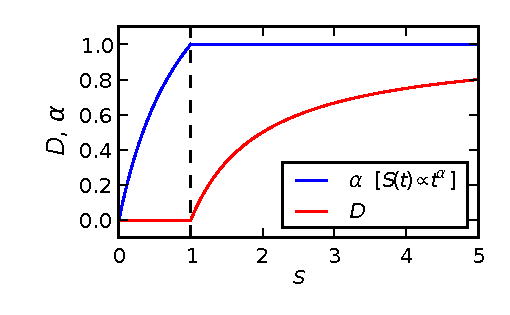
\includegraphics[width=0.45\textwidth]{alexander}
  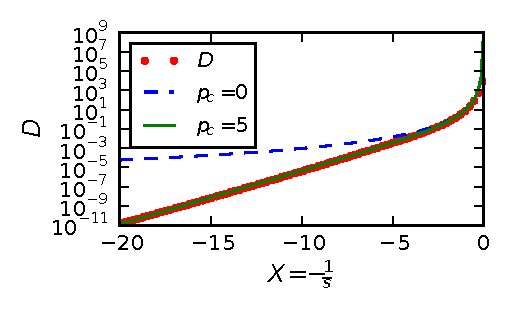
\includegraphics[width=0.45\textwidth]{ERH}
\caption{The zero activation energy model: (left) The dependence of $D$ and $\alpha$ on $s$ 
as predicted by the theory for a $1D$ network. (right) Numerical resuls for $D$ in the case of a $2D$ network, based on spectral analysis of Fig\ref{fig:spectral}  compared with our ERH prediction. The dashed line is LRT.}
\label{fig:alexander}
\end{figure}

  }





%%%%%%%%%%%%%%%%%%%%%%%%%%%%%%%%%%%%%%%%%%%%%%%%%%%%%%%%%%%%%%%%%%%%%%%%%%%%%%
  \headerbox{Eigenvalue distributions}{name=eigvals,column=1,span=2, below=alexander}{
%%%%%%%%%%%%%%%%%%%%%%%%%%%%%%%%%%%%%%%%%%%%%%%%%%%%%%%%%%%%%%%%%%%%%%%%%%%%%%
%%%%%%%%%%%%%%%%%%5
\begin{figure}[H]
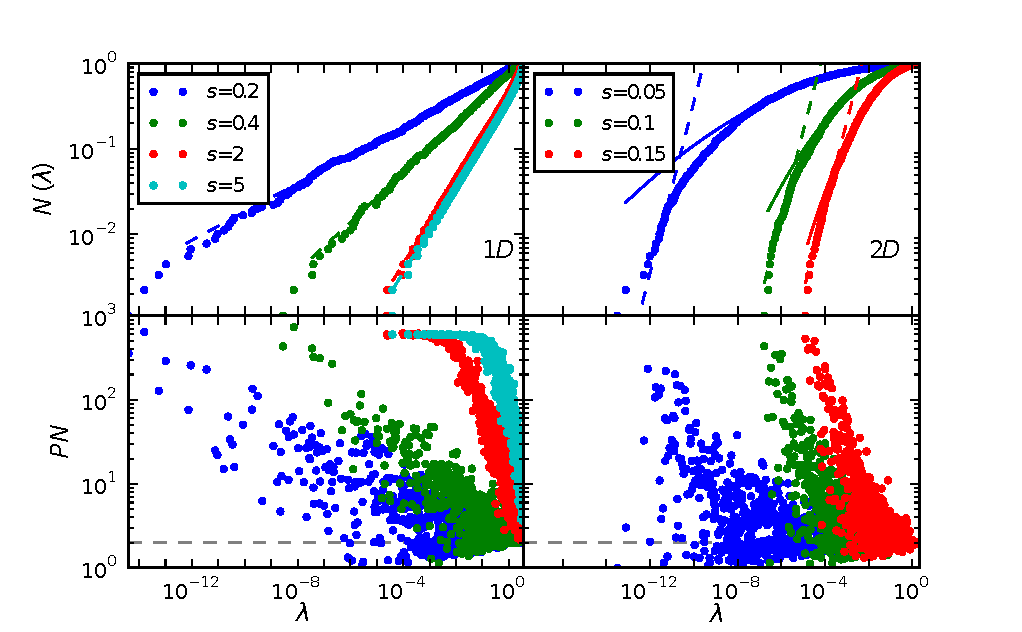
\includegraphics[clip, width=0.95\textwidth]{four_panels}
\caption{ Spectral properties for $1D$ and $2D$. The upper panels show the cumulative count of the eigenvalues, while the lower panels present the participation number of the corresponding eigenmodes. In the $2D$ case the RG analysis of the localized modes \cite{amir} predicts the solid lines. The numerics show clearly a departure towards a diffusive behavior, as implied by ERH.} \label{fig:spectral}
\end{figure}
}


%%%%%%%%%%%%%%%%%%%%%%%%%%%%%%%%%%%%%%%%%%%%%%%%%%%%%%%%%%%%%%%%%%%%%%%%%%%%%%
  \headerbox{Banded Lattice Model}{name=banded,column=1,span=2, below=eigvals,above=refs}{
%%%%%%%%%%%%%%%%%%%%%%%%%%%%%%%%%%%%%%%%%%%%%%%%%%%%%%%%%%%%%%%%%%%%%%%%%%%%%%
\begin{figure}[H]
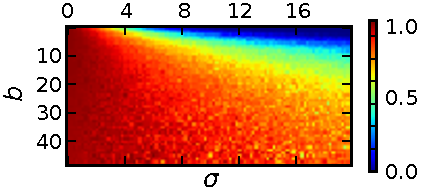
\includegraphics[height=10em]{resnet_new}
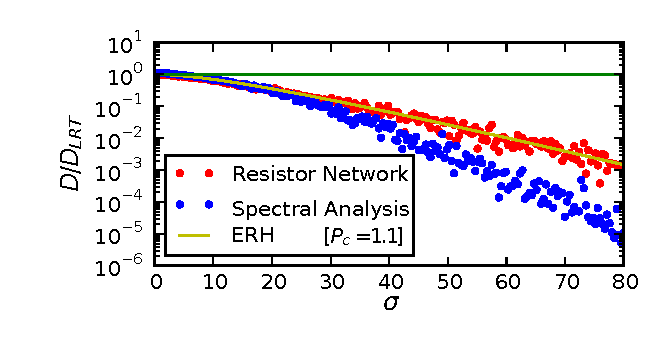
\includegraphics[height=10em]{banded_b10}
\caption{(left) The numerical result for $D/D_{\tbox{LRT}}$ imaged as a function of $\sigma$ and $b$. (right) Plot of the results for a $b=10$ matrix. The blue points are based on spectral analysis (involving an undeterminded pre-factor). The curve is our ERH prediction.}
\end{figure}

}



\end{poster}

\end{document}
